\documentclass[12pt,a4paper]{article}
\usepackage[utf8]{inputenc}
\usepackage[T1]{fontenc}
\usepackage{amsmath}
\usepackage{amsfonts}
\usepackage{amssymb}
\usepackage{graphicx}
\usepackage{geometry}
\geometry{left=2.5cm,right=2.5cm,top=1.0cm,bottom=1.5cm}

\usepackage{amsmath}
\usepackage{enumerate}
\usepackage{booktabs}

%minted --insert code
\usepackage{minted}
\usepackage{xcolor}
\definecolor{background-color}{HTML}{f3f3f3} %background-color
\newcommand{\inputmintedfile}[2]{
\inputminted[linenos=true,
bgcolor=background-color,
fontsize= \footnotesize,
fontfamily=courier ,
breaklines=true
]{#1}
{#2}
}
%algorithm redefine
\usepackage{algorithm}
\usepackage{algorithmicx}
\usepackage{algpseudocode}
\renewcommand{\algorithmicrequire}{\textbf{Input:}}
\renewcommand{\algorithmicensure}{\textbf{Output:}}


\author{Zuyao Chen   201728008629002 \\zychen.uestc@gmail.com}
\title{Homework1}
\date{}

\begin{document}
\maketitle

\section{Question1}
\begin{enumerate}[a).]
\item  \textbf{algorithm description:} \\	
Let ``query($X,k$)'' denotes the $k^{th}$ smallest number of $A$ or $B$ and 
we call two databases $A=\{a_1,a_2,...,a_i,...,a_n\},B=\{b_1,b_2,...,b_j,...,b_n\}$ arranged in
ascending order
(In fact,it does no matter to care the sequence order owing to ``query''  ).\\
$\text{query}(A,i)$ can be written as $a_i$,as well as $\text{query}(B,j)$.
Making sure $i+j=n$ , 
\begin{itemize}
	\item  if $a_i < b_j$, the median lies in $\{a_{i+1},...,a_n\} \bigcup \{b_1,b_2,...,b_j\}$;
	\item  if $a_i = b_j$, the median is $a_i$ or $b_j$;
	\item  if $a_i > b_j$, the median lies in $\{a_1,a_2,...,a_i\} \bigcup \{b_{j+1},...,b_n \}$
\end{itemize}
We initialize $i = n/2, j = n -i$,that equals to comparing the median of each database.
Then the search area can be narrowed down to half length of the last
until we just need to find $1^{th}$ smallest number between two separate arrays. \\
pseudo-code:
\begin{algorithm}[H]
\caption{finding the median of two separate databases via query}
\begin{algorithmic}[1]
\Require Two separate databases $A$,$B$,length $n$. (initializing $i,j=0,k=n$)	
\Ensure  the median(the $n^{th}$ smallest) of $A\bigcup B$
\Function {find\_kth}{$A,i,B,j,k$}
\If {$k = 1$}
\State \Return $\min \{\text{query}(A,i+1),\text{query}(B,j+1)
		\} $
\EndIf
\If {$i = 0$ (initial)}
\State $i \gets k/2, j \gets k - i$
\EndIf
\If {$\text{query}(A,i) < \text{query}(B,j)$}
\State $ k \gets k - k/2$ (each discards $k/2$ numbers)
\State $ i \gets i + k/2, j \gets j - k/2$
\If {$k=1$}
\State $j \gets j-1$
\EndIf

\State \Return \Call{find\_kth}{$A,i,B,j,k$}
\ElsIf {$\text{query}(A,i) > \text{query}(B,j)$}
\State $k \gets k-k/2,i \gets i - k/2,j \gets j + k/2$
\If {$k=1$}
\State $i \gets i-1$
\EndIf
\State \Return \Call{find\_kth}{$A,i,B,j,k$}
\Else
\State \Return $\text{query}(A,i)$
\EndIf
\EndFunction
\end{algorithmic}	
\end{algorithm}

\item \textbf{subproblem reduction graph}
\begin{figure}[H]
\centering
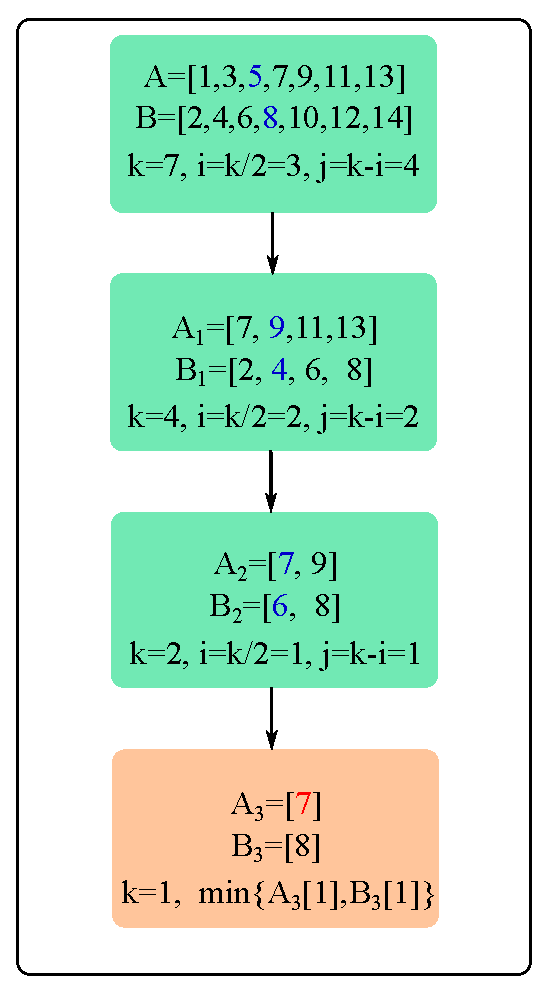
\includegraphics[width=0.45\textwidth,height=0.4\textheight]{pictures/graph_median}	
\caption{problem instance}
\end{figure}
\item \textbf{proof of the correctness} \\
%it may be difficult...
Obviously, $k = 1$ means that we just want the $1^{th}$ smallest number of
$A\bigcup B$.
In order to find the median of $A\bigcup B$,we initialize $i = n/2, j= n-i, k = n$.
Let ``$A[i]$'' denotes ``$\text{query}(A,i)$'',
then compare $A[i]$ with $B[j]$: 
\begin{enumerate}[i.]
	\item   if $A[i] < B[j]$, we can surely say that $\{A[1],A[2],...,A[i]\}$ must lies in the left of 
		  the median and $\{B[j+1],...,B[n]\}$ must lies in the right of the median.For instance,
		  if $B[j+1]$ is the median,then there has $i+j=n$ numbers smaller than $B[j+1]$
		   (each element of $\{A[1],...,A[i]\}\cup \{B[1],B[2],...,B[j]\}$ is smaller than $B[j+1]$
		   ).
	\item if $A[i] = B[j]$, the median is $A[i]$ (or $B[j]$).
	\item if $A[i] > B[j]$,it's the opposite of i. 	   		   
\end{enumerate}
in each iteration, we discard $k/2$ numbers until $k=1$.	

\item \textbf{complexity of the algorithm}  \\
The size of original problem is reduced to half at each iteration,
and ``query'' costs $O(1)$,thus \\
\[
T(n) = T(n/2) + cO(1) = O(\log n)
\]
	
\end{enumerate}
\section{Question2}
\begin{enumerate}[a).]
\item  \textbf{algorithm description:}
\begin{itemize}
	\item first,we randomly choose $v$ from the array $A$;
	\item second,we split $A$ into three categories : elements greater than $v$,
	those equal to $v$,and those smaller than $v$.Call these $A_L,A_v,A_R$ respectively.
	\item then,we have 
	\begin{equation*}
	 \text{select}(A,k) = \left\lbrace 
	 \begin{array}{lll}
	 \text{select}(A_L,k) &\text{if}& k \leq  \text{len}(A_L)\\
	 v  &\text{if}& \text{len}(A_L) < k \leq \text{len}(A_L) + \text{len}(A_v)\\
	 \text{select}(A_R,k-\text{len}(A_L)-\text{len}(A_v)) &\text{if}& k > \text{len}(A_L) + \text{len}(A_v)
	 \end{array}
	 \right.
	\end{equation*}
	here ``len'' represents the length of an array.
\end{itemize}
pseudo-code:
\begin{algorithm}
\caption{find the $k^{th}$ largest element in an unsorted array}
\begin{algorithmic}[1]
\Require An unsorted array $A$ and $k$
\Ensure the $k^{th}$ largest number	of  $A$
\Function{select}{$A,k$}
\If {$k \leq 0$ or $k > \text{len}(A)$} 
\State \Return error
\EndIf
\State randomly choose $v$ of $A$
\State $A_L=\{\},A_v=\{\},A_R=\{\}$
\For {$i = 1 $ to $\text{len}(A)$} 
\If {$A[i] > v$}
\State $A_L = A_L \bigcup \{A[i]\} $
\ElsIf {$A[i] = v$}
\State $A_v = A_v \bigcup \{A[i]\} $
\Else
\State $A_R = A_R \bigcup \{A[i]\} $
\EndIf
\EndFor
\If {$k \leq \text{len}(A_L)$}
\State \Return \Call{select}{$A_L,k$}
\ElsIf {$k \leq \text{len}(A_L) + \text{len}(A_v)$}
\State \Return $v$ 
\Else
\State \Return \Call{select}{$A_R,k- \text{len}(A_L) - \text{len}(A_v)$}
\EndIf
\EndFunction
\end{algorithmic}
\end{algorithm}
\item  \textbf{subproblem reduction graph}
\begin{figure}[H]
\centering
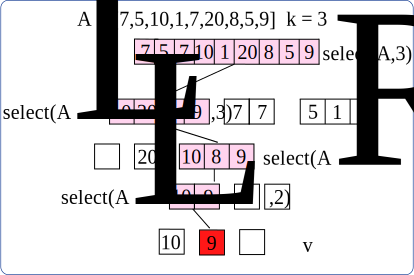
\includegraphics[width = 0.6\textwidth,height=0.25\textheight]{pictures/graph1}
\caption{problem instance}
\end{figure}
\item \textbf{proof of the correctness} \\
In terms of the input constraints, it should throw an exception given $k \leq 0 $ or $k > \text{len}(A)$.
What we want is finding the $k^{th}$ largest number of array $A$,there is no need to sort the array.
In every recursion, the search can be narrowed down to one of three sublists until we choose the correct one of 
singletons.

\item \textbf{complexity of the algorithm} \\
Splitting $A$ into three parts costs linear time.
\begin{itemize}
	\item The most worst situation is that we choose the smallest  number every times,
	then it would force our algorithm to perform \\
	\[
	T(n) = T(n-1) + O(n)
	\]
	or $O(n^{2})$ operations.
	\item The best-case scenario is that we select the median at each iteration,
	thus it would perform \\
	\[
	T(n) = T(n/2) + O(n) 
	\]
	or $O(n)$ operations.
	\item good choice: select a nearly-central element ,
		$\text{len}(A_L) \geq \epsilon \text{len}(A)$,$
		\text{len}(A_R) \geq \epsilon \text{len}(A)$ for a fixed $0 < \epsilon < 1$,
	\begin{align*}
	T(n) \leq &T((1-\epsilon)\text{len}(A)) + O(n) \\
	 \leq &cn + c(1-\epsilon)n + c(1-\epsilon)^{2}n + ... \\
	 =& O(n)
	\end{align*}	
			
	
\end{itemize} 




\end{enumerate}	
	

\section{Question3}
\begin{enumerate}[a).]
\item  \textbf{algorithm description:}



\item  \textbf{subproblem reduction graph}
	
\item \textbf{proof of the correctness}	


\item \textbf{complexity of the algorithm}	
\end{enumerate}

	
\section{Question5}
\qquad well,it's a second bracketing problem and the answer is a \textbf{Catalan number}.
I don't know how to analysis it  using the method of divide and conquer,
so I just put up the implementation of the math formula:
\begin{equation*}
\text{tri}(n) = \text{tri}(2)*\text{tri}(n-1) + \text{tri}(3)*\text{tri}(n-2) + ... +\text{tri}(n-1)*\text{tri}(2)
\end{equation*} 
where $\text{tri}(2) = \text{tri}(3) = 1$,$\text{tri}(n)$ represents the number of triangulations of a convex polygon with $n$ vertices.
%\inputmintedfile{c++}{../c_plus_plus/triangulations.cpp}
the test result is showed below: \\
\begin{table}[H]
	\centering
	\begin{tabular}{ccc}
	\toprule
	n & tri(n) \\
	\midrule
	3 &	1 \\
	4 &	2 \\
	5 &	5 \\
	6 &	14 \\
	7 &	42 \\
	8 &	132 \\
	\bottomrule
	\end{tabular}
	\qquad 
	\begin{tabular}{ccc}
	\toprule
	n & tri(n) \\
	\midrule
	9 &	429 \\
	10 &1430 \\
	11 &486 \\
	12 &16796 \\
	13 &58786 \\
	14 & 208012 \\
	\bottomrule	
	\end{tabular}
	\caption{test result}
\end{table}
Obviously,the complexity of the algorithm is $O(n^{2})$.
\section{Question8}
\qquad It's impossible to use Quick-Sort,because Quick-Sort will lose some 
information about sequence.
%----insert cpp ---
\inputmintedfile{c++}{../c_plus_plus/count_inversions.cpp}
\section{Question9}
%\lstinputlisting{../c_plus_plus/closest_pair.cpp}
%---use minted ---
%\inputminted[linenos=true,
%bgcolor=background-color,
%fontsize=\footnotesize,
%fontfamily=courier ,
%breaklines=true
%]{c++}
%{../c_plus_plus/closest_pair.cpp}
\inputmintedfile{c++}{../c_plus_plus/closest_pair.cpp}	
	
\end{document}